\todo{
zins
avols para la fleischer
simulaciones y mediciones
histogramas (?????)
eleccion de componentes
aprox cheby
RANGO DINAMICO
limitaciones tension de entrada
pcb
}

\section{Celdas Universales}

En esta secci\'on se analizan distintas celdas universales, es decir, celdas de configuraciones diferentes que est\'an compuestas por dos integradores. Las celdas en estudio son la Kerwin-Huelsman-Newcomb, la Tow-Thomas, la Ackerberg-Mossberg y la Fleischer-Tow. La finalidad de dicho an\'alisis es luego realizar un filtro rechaza banda a partir de una aproximaci\'on de Chebychev Inverso que cumpla las siguientes especificaciones:

	\begin{table}[H]
	\centering
	\begin{tabular}{c c}
		\hline
		$f_\infty$ & $51kHz$ \\ 
		notch depth &  $\geq 50dB$\\
		$\Delta f_a$ & $600Hz$\\
		$\Delta f_p$ & $10kHz$\\
		$A_a$ & $40dB$\\
		$A_p$ & $6dB$\\
		$G$ & $[-3:3]dB$\\
		$|Zin(f)|$ & $\geq 50k\Omega$\\	
		Cantidad de ceros de transmisi\'on & $\geq 2$\\
		\hline
	\end{tabular}
	\caption{Especificaciones del filtro rechaza banda a realizar.}
	\label{especificaciones}
\end{table}

El an\'alisis que se llevar\'a a cabo para cada celda es tanto ideal como real, para poder comprender las caracter\'isticas que determinar\'an si es posible o no implementar cada celda para lograr el filtro especificado. Una vez determinadas las ventajas y desventajas de cada celda frente al filtro que se desea realizar, se har\'a un mayor enfoque en la celda elegida para llevar el filtro a la pr\'actica.


\subsection{Configuraciones correspondientes a distintas celdas universales: An\'alisis ideal}

A continuaci\'on se detallan las configuraciones de las cuatro celdas universales previamente enunciadas. Junto a la configuraci\'on circuital de cada una de estas celdas, se presenta su funci\'on transferencia, la ganancia $G$, los par\'ametros $Q$ y $\omega_0$; y sus sensibilidades relativas respecto a cada componente que conforma el circuito. Para esto, se hace un an\'alisis en el que los amplificadores operacionales son considerados ideales. Es decir, se considera que cada amplificador operacional cuenta con las siguientes caracter\'isticas:

\begin{equation}
	\begin{cases}
		Z_{in} \to \infty\\
		A_{VOL} \to \infty\\
		Z_{out} \to 0\Omega\\
		I_{in+} = I_{in-} = 0A
		
	\end{cases}
\end{equation}


\todo{citar la pagina esta de internet}
\footnote{https://elxcompacme.files.wordpress.com/2014/03/filter-kendell-su.pdf}
\subsection{Celda 2do orden Kerwin-Huelsman-Newcomb (KHN): An\'alisis ideal}


\begin{figure}[H] %!ht
	\centering
	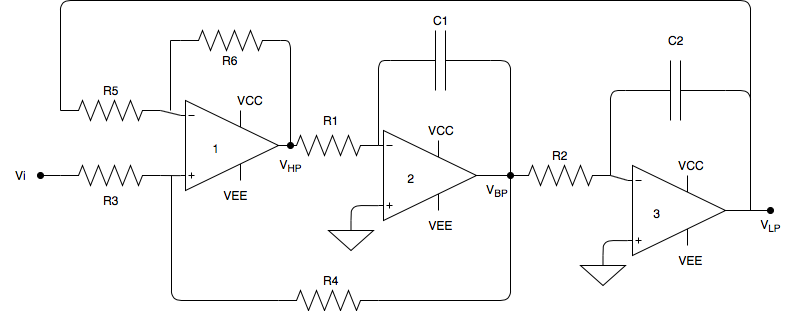
\includegraphics[width=12cm,height=12cm,keepaspectratio]{../EJ4/imagenes/KERWIN.png}
	\caption{Circuito Kerwin-Huelsman-Newcomb}
	\label{kerwin}
\end{figure}

\subsubsection{Funci\'on transferencia y par\'ametros}
\begin{table}[h!]
	\centering
	\begin{tabular}{c c c c c}
		Salida & $H(s)$ & $G$ & $\omega_0$ & $Q$\\
		\hline \\
		LP & $\frac{\frac{R_4}{R_5R_1R_2C_1C_2}\cdot \frac{R_5+R_6}{R_3+R_4}}{S^2+\frac{R_3}{R_5R_1C_1}\cdot \frac{R_5+R_6}{R_3+R_4}s+\frac{R_6}{R_5R_1R_2C_1C_2}}$& $\frac{R_4 (R_5+R_6)}{R_6(R_3+R_4)}$& \multirow{7}{*}{$\sqrt{\frac{R_4 (R_5+R_6)}{R_6(R_3+R_4)}}$}&
		\multirow{7}{*}{$\frac{R_5(R_3+R_4)}{R_3(R_5+R_6)}\cdot \sqrt{\frac{R_6R_1C_1}{R_5R_2C_2}}$}\\ \\
		BP & $- \frac{\frac{R_4}{R_5R_1C_1}\cdot \frac{R_5+R_6}{R_3+R_4} s}{S^2+\frac{R_3}{R_5R_1C_1}\cdot \frac{R_5+R_6}{R_3+R_4}s+\frac{R_6}{R_5R_1R_2C_1C_2}}$&$-\frac{R_4}{R_3}$& &\\ \\
		HP& $- \frac{\frac{R_4}{R_5}\cdot \frac{R_5+R_6}{R_3+R_4} S^2}{S^2+\frac{R_3}{R_5R_1C_1}\cdot \frac{R_5+R_6}{R_3+R_4}s+\frac{R_6}{R_5R_1R_2C_1C_2}}$& $\frac{R_4(R_5+R_6)}{R_5(R_3+R_4)}$& & \\ \\
		\hline
	\end{tabular}
	\caption{Caracter\'isticas de la celda Kerwin-Huelsman-Newcomb.}
	\label{hg_tt}
\end{table}

\subsubsection{Sensibilidades}

\begin{table}[H]
	\centering
	\begin{tabular}{c c c c c c}
		  & $\omega_0$ & $Q$ &$G_{LP}$ & $G_{BP}$& $G_{HP}$\\
		\hline \\
	$R_1$ & $-\frac{1}{2}$& $\frac{1}{2}$ & $0$& $0$&$0$\\ \\
	$R_2$ & $-\frac{1}{2}$& $-\frac{1}{2}$ & $0$& $0$& $0$\\ \\
	$R_3$ & $0$& $-\frac{R_4}{R_3+R_4}$ & $-\frac{R_3}{R_3+R_4}$&$-1$ & $-\frac{R_3}{R_3+R_4}$\\ \\
	$R_4$ & $0$& $\frac{R_4}{R_3+R_4}$& $\frac{R_3}{R_3+R_4}$ &$1$ & $\frac{R_3}{R_3+R_4}$\\ \\
	$R_5$ & $-\frac{1}{2}$&$\frac{R_6-R_5}{2(R_5+R_6)}$ & $\frac{R_5}{R_5+R_6}$&$0$ & $-\frac{R_6}{R_5+R_6}$\\ \\
	$R_6$ & $\frac{1}{2}$& $-\frac{R_6-R_5}{2(R_5+R_6)}$ & $-\frac{R_5}{R_5+R_6}$& $0$&$\frac{R_6}{R_5+R_6}$ \\ \\
	$C_1$ & $-\frac{1}{2}$& $\frac{1}{2}$ & $0$& $0$&$0$ \\ \\
	$C_2$ & $-\frac{1}{2}$& $-\frac{1}{2}$ & $0$ & $0$&$0$\\ \\
		\hline
	\end{tabular}
	\caption{Sensibilidades de la celda Kerwin-Huelsman-Newcomb.}
	\label{sens_k}
\end{table}


Esta celda tiene sensibilidades bajas.

\subsubsection{Impedancia de entrada}
\todo{completar}


\subsubsection{Impedancia de salida}
La salida del circuito se encuentra a la salida de un amplificador operacional con realimentaci\'on negativa.  Se indic\'o previamente que la impedancia de salida de un amplificador operacional ideal es $Z_{out} \to 0$, lo que implica que la impedancia de salida del circuito tambi\'en tienda a cero.

\begin{equation}
\begin{cases}
Vo_2 = -\frac{1}{2} \cdot Vo_1\\
Vo_3 = -\frac{1}{2} \cdot Vo_2\\
H(s) = \frac{Vo_3}{V_i} = G \cdot \frac{a_0}{s^2 + b_1 s + b_0}
\label{int2eq}
\end{cases}
\end{equation}

Dependiendo de d\'onde se tome la salida del circuito \ref{kerwin}, se puede obtener un filtro pasa altos, un pasa banda o un pasabajos. Lo que sucede con Kerwin-Huelsman-Newcomb es que no brinda una salida rechaza banda. La misma puede igual lograrse agregandole al circuito \ref{kerwin} un sumador, como se muestra en la figura \ref{sumador_extra}:

\begin{figure}[H] %!ht
	\centering
	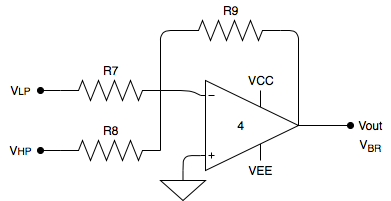
\includegraphics[width=8cm,height=8cm,keepaspectratio]{../EJ4/imagenes/sumador_extra.png}
	\caption{Sumador que se le agrega a la selda para obtener un rechaza banda.}
	\label{sumador_extra}
\end{figure}

\subsection{Celda 2do orden Tow-Thomas:An\'alisis ideal}

La celda Tow-Thomas var\'ia frente a la Kerwin-Huelsman-Newcomb al tener juntos a la entrada el sumador y el primer integrador, agregando luego un inversor y una resistencia en la realimentación que va de la salida $V_{LP}$ a la entrada del circuito. Esta nueva configuraci\'on, al igual que en la Kerwin-Huelsman-Newcomb sigue teniendo una salida de pasa bajos y una de pasa banda, pero ya no tiene una de pasa altos. 

\begin{figure}[H] %!ht
	\centering
	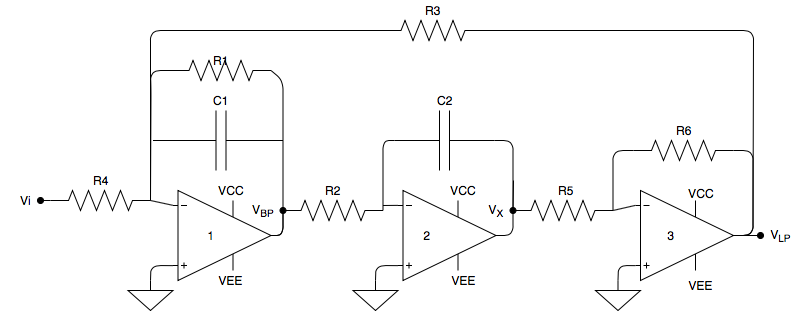
\includegraphics[width=12cm,height=12cm,keepaspectratio]{../EJ4/imagenes/TOW-THOMAS.png}
	\caption{Celda Tow-Thomas}
	\label{tow_thomas}
\end{figure}

\subsubsection{Funci\'on transferencia y par\'ametros}
Los par\'ametros correspondientes a la celda Tow-Thomas son los siguientes:

\begin{table}[H]
	\centering
	\begin{tabular}{c c c c c}
		Salida & $H(s)$ & $G$ & $\omega_0$ & $Q$\\
		\hline \\
		LP & $-\frac{\frac{R_6/R_5}{R_2R_4C_1C_2}}{s^2+\frac{1}{R_1C_1}+\frac{R_6/R_5}{R_2R_3C_1C_2}}$& $- \frac{R_3}{R_4}$& \multirow{4}{*}{$\sqrt{\frac{R_6/R_5}{R_2R_3C_1C_2}}$}&
		\multirow{4}{*}{$\frac{R_1}{\sqrt{R_2R_3}}\sqrt{\frac{R_6C_1}{R_5C_2}}$}\\ \\
		BP & $-\frac{\frac{1}{R_4 C_1}s}{s^2+\frac{1}{R_1C_1}+\frac{R_6/R_5}{R_2R_3C_1C_2}}$&$-\frac{R_1}{R_4}$& &\\ \\
		\hline
	\end{tabular}
	\caption{Caracter\'isticas de la celda Tow-Thomas.}
	\label{hg_tt}
\end{table}

\subsubsection{Sensibilidades}
\begin{table}[H]
	\centering
	\begin{tabular}{c c c c c }
		& $\omega_0$ & $Q$ &$G_{LP}$ & $G_{BP}$\\
		\hline \\
		$R_1$ & $0$& $1$ & $0$& $1$\\ \\
		$R_2$ & $-\frac{1}{2}$& $-\frac{1}{2}$ & $0$& $0$\\ \\
		$R_3$ & $-\frac{1}{2}$& $-\frac{1}{2}$ & $1$&$0$ \\ \\
		$R_4$ & $0$& $0$& $-1$ &$-1$ \\ \\
		$R_5$ & $-\frac{1}{2}$&$-\frac{1}{2}$ & $0$&$0$ \\ \\
		$R_6$ & $\frac{1}{2}$& $\frac{1}{2}$ & $0$& $0$ \\ \\
		$C_1$ & $-\frac{1}{2}$& $\frac{1}{2}$ & $0$& $0$\\ \\
		$C_2$ & $-\frac{1}{2}$& $-\frac{1}{2}$ & $0$ & $0$\\ \\
		\hline
	\end{tabular}
	\caption{Sensibilidades de la celda Tow-Thomas.}
	\label{sens_tt}
\end{table}

\subsubsection{Impedancia de entrada}
\todo{COMPLETAR}

\subsubsection{Impedancia de salida}
Al igual que para la celda anterior, como la impedancia de salida del circuito es tomada a la salida de un amplificador operacional y dado que este es considerado ideal, la impedancia de salida del circuito tiende a cero.

\subsection{Celda 2do orden Ackerberg-Mossberg: An\'alisis ideal}

\begin{figure}[H] %!ht
	\centering
	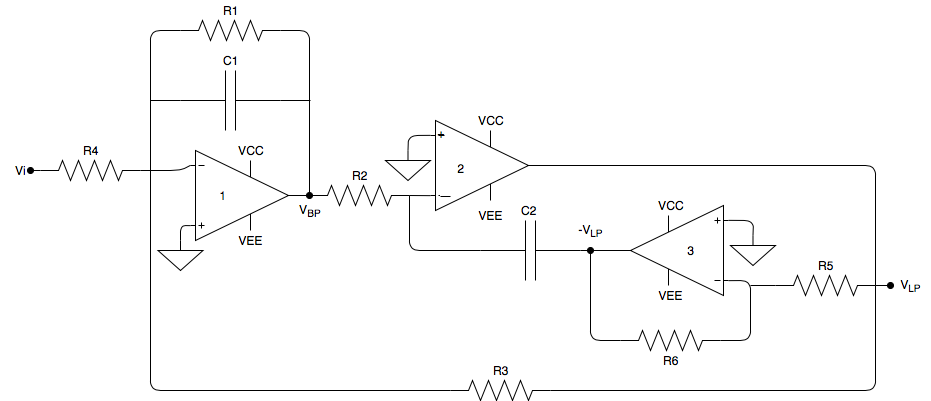
\includegraphics[width=12cm,height=12cm,keepaspectratio]{../EJ4/imagenes/ACKBERG.png}
	\caption{Celda Ackerberg-Mossberg}
	\label{ackerberg}
\end{figure}

\subsubsection{Funci\'on transferencia y par\'ametros}

\begin{table}[H] %estas son las del libro!
	\centering
	\begin{tabular}{c c c c c}
		Salida & $H(s)$ & $G$ & $\omega_0$ & $Q$\\
		\hline \\
		LP & $- \frac{\frac{R_5}{C_1C_2R_2R_4R_6}}{s^2+\frac{1}{C_1R_1}s+\frac{R_5}{C_1C_2R_2R_3R_6}}$& $-\frac{R_3}{R_4}$& \multirow{4}{*}{$\sqrt{\frac{R_5}{C_1C_2R_2R_3R_6}}$}&
		\multirow{4}{*}{$C_1R_1\sqrt{\frac{R_5}{C_1C_2R_2R_3R_6}}$}\\ \\
		BP & $-\frac{\frac{1}{C_1R_4}s}{s^2+\frac{1}{C_1R_1}s + \frac{R_5}{C_1C_2R_2R_3R_6}}$&$-\frac{R_1}{R_4}$& &\\ \\
		\hline
	\end{tabular}
	\caption{Caracter\'isticas de la celda Ackerberg-Mossberg.}
	\label{am_tt}
\end{table}

\subsubsection{Sensibilidades}

\begin{table}[H]
	\centering
	\begin{tabular}{c c c c c }
		& $\omega_0$ & $Q$ &$G_{LP}$ & $G_{BP}$\\
		\hline \\
		$R_1$ & $0$ & $1$ & $0$ & $1$\\ \\
		$R_2$ & $-\frac{1}{2}$ & $-\frac{1}{2}$ & $0$ & $0$\\ \\
		$R_3$ & $-\frac{1}{2}$ & $-\frac{1}{2}$ & $1$ & $0$ \\ \\
		$R_4$ & $0$ & $0$ & $-1$ & $-1$ \\ \\
		$R_5$ & $\frac{1}{2}$ & $\frac{1}{2}$ & $0$ & $0$ \\ \\
		$R_6$ & $-\frac{1}{2}$ & $-\frac{1}{2}$ & $0$ & $0$ \\ \\
		$C_1$ & $-\frac{1}{2} $ & $\frac{1}{2}$ & $0$ & $0$\\ \\
		$C_2$ & $-\frac{1}{2}$ & $-\frac{1}{2}$ & $0$ & $0$\\ \\
		\hline
	\end{tabular}
	\caption{Sensibilidades de la celda Ackerberg-Mossberg.}
	\label{sens_am}
\end{table}

\subsubsection{Impedancia de entrada}
\todo{completar}

\subsubsection{Impedancia de salida}
Esta celda tambi\'en presenta una impedancia de salida igual a cero al considerar los amplificadores operacionales como ideales, debido a que la salida del circuito es tomada a la salida de un amplificador operacional.

\subsection{Celda 2do orden Fleischer-Tow: An\'alisis ideal}

Una caracter\'istica importante a remarcar de la selda Flesicher-Tow es que, a diferencia de las celdas anteriores, permite realizar cualquier tipo de filtro de segundo orden sin la necesidad de agregar otro amplificador operacional. Como se ha estudiado en trabajos pr\'acticos anteriores, el amplificador operacional tiene ciertas limitaciones para un circuito, debidas al slew rate, a la saturaci\'on, entre otras; por lo que es ventajoso el hecho de no tener que agregar un amplificador operacional para obtener un filtro rechaza banda.


\begin{figure}[H] %!ht
	\centering
	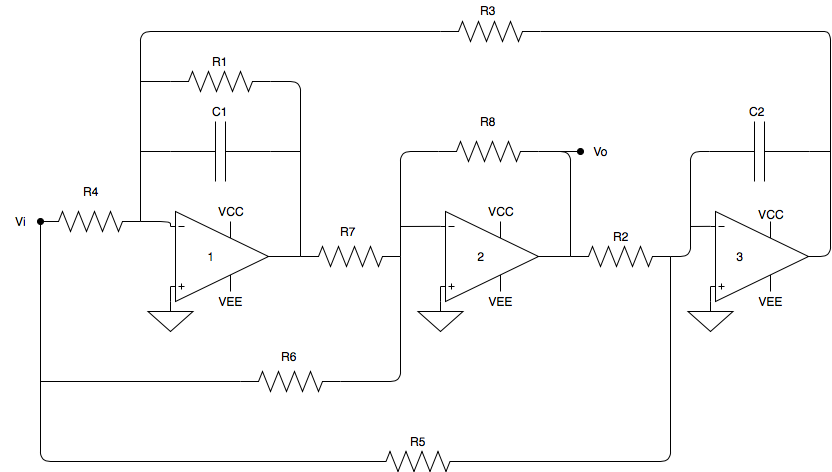
\includegraphics[width=12cm,height=12cm,keepaspectratio]{../EJ4/imagenes/FLEISCHER.png}
	\caption{Celda Fleischer-Tow}
	\label{fleischer}
\end{figure}

\subsubsection{Funci\'on transferencia y par\'ametros}

\begin{table}[H] %estas son las del libro!
	\centering
	\begin{tabular}{c c c c}
		$H(s)$ gen\'erica & $\omega_0$ & $Q$\\
		\hline \\
		 $- \frac{\frac{R_8}{R_6}s^2+\left(\frac{R_8}{R_6R_1C_1}-\frac{R_8}{R_4R_7C_1}\right)s+\frac{R_8}{R_3R_5R_7C_1C_2}}{s^2+\frac{1}{R_1C_1}s+\frac{R_8}{R_2R_3R_7C_1C_2}}$&$\sqrt{\frac{R_8}{R_2R_3R_7C_1C_2}}$&$R_1C_1\sqrt{\frac{R_8}{R_2R_3R_7C_1C_2}}$\\ \\
		\hline
	\end{tabular}
	\caption{Expresiones gen\'ericas de la celda Fleischer-Tow.}
	\label{f_generica}
\end{table}

\begin{table}[H] %estas son las del libro!
	\centering
	\begin{tabular}{c c c c c c c}
		Salida & Condiciones & $H(s)$ & $G$ & $\omega_p$ & $Q$ & $\omega_z$\\
		\hline \\
		LP&$R_6=R_4=\infty$ &$- \frac{\frac{R_8}{R_3R_5R_7C_1C_2}}{s^2+\frac{1}{R_1C_1}s+\frac{R_8}{R_2R_3R_7C_1C_2}}$& $-\frac{R_2}{R_5}$& \multirow{9}{*}{$\sqrt{\frac{R_8}{R_2R_3R_7C_1C_2}}$}&
		\multirow{9}{*}{$R_1C_1\sqrt{\frac{R_8}{R_2R_3R_7C_1C_2}}$} &\multirow{9}{*}{$\sqrt{\frac{R_6}{R_3 R_5 R_7 C_1 C_2}}$}\\ \\
		BP &$R_6=R_5=\infty$  &$ \frac{\left(\frac{R_8}{R_4R_7C_1}\right)s}{s^2+\frac{1}{R_1C_1}s+\frac{R_8}{R_2R_3R_7C_1C_2}}$&$\frac{R_1R_8}{R_4R_7}$& & &\\ \\
		HP & $R_5=\infty$&\multirow{2}{*}{$- \frac{\frac{R_8}{R_6}s^2}{s^2+\frac{1}{R_1C_1}s+\frac{R_8}{R_2R_3R_7C_1C_2}}$}&\multirow{2}{*}{$-\frac{R_8}{R_6}$}& & &\\ 
		&$R_1R_6=R_4R_7$ & & & & &\\ \\
		BR &$R_1R_6=R_4R_7$ &\multirow{2}{*}{$- \frac{\frac{R_8}{R_6}s^2+\frac{R_8}{R_3R_5R_7C_1C_2}}{s^2+\frac{1}{R_1C_1}s+\frac{R_8}{R_2R_3R_7C_1C_2}}$}&\multirow{2}{*}{$-\frac{R_2}{R_5}$}& & & \\ \\ \\
		\hline
	\end{tabular}
	\caption{Caracter\'isticas de la celda Fleischer-Tow.}
	\label{f_cars}
\end{table}

\subsubsection{Sensibilidades}

\begin{table}[H]
	\centering
	\begin{tabular}{c c c c c c c}
		& $\omega_0$ & $Q$ &$G_{LP}$ & $G_{BP}$& $G_{HP}$& $G_{BR}$\\
		\hline \\ 
		$R_1$ & $0$ & $1$ & $0$ & $1$ & $0$ & $0$\\ \\
		$R_2$ & $-\frac{1}{2}$ & $-\frac{1}{2}$ & $1$ & $0$ & $0$ & $1$\\ \\
		$R_3$ & $-\frac{1}{2}$ & $-\frac{1}{2}$ & $0$ & $0$ & $0$ & $0$\\ \\
		$R_4$ & $0$ & $0$ & $0$ & $-1$ & $0$ & $0$\\ \\
		$R_5$ & $0$ & $0$ & $-1$ & $0$ & $0$ & $-1$\\ \\
		$R_6$ & $0$ & $0$ & $0$ & $0$ & $-1$ & $0$\\ \\
		$R_7$ & $-\frac{1}{2}$ & $-\frac{1}{2}$ & $0$ & $-1$ & $0$ & $0$\\ \\
		$R_8$ & $\frac{1}{2}$ & $\frac{1}{2}$ & $0$ & $1$ & $1$ & $0$\\ \\
		$C_1$ & $-\frac{1}{2}$ & $\frac{1}{2}$ & $0$ & $0$ & $0$ & $0$\\ \\
		$C_2$ & $-\frac{1}{2}$ & $-\frac{1}{2}$ & $0$ & $0$ & $0$ & $0$\\ \\
		\hline
	\end{tabular}
	\caption{Sensibilidades de la celda Fleischer-Tow}
	\label{sens_am}
\end{table}

\subsubsection{Impedancia de entrada}
Al considerar los amplificadores operacionales como ideales, la impedancia de entrada a los mismos es infinita mientras que su impedancia de salida es cero. Tambi\'en se toma como masa virtual a la terminal de entrada negativa del amplificador operacional ideal ya que sigue a la de la entrada positiva, la cual es Tierra. Para calcular la impedancia de entrada de la celda, se tomaron las siguientes relaciones:

\begin{equation}
	\begin{cases}
		Z_in = \frac{V_i}{I_i}\\
		I_i = I_4 + I_5 + I_6\\
		I_4 = \frac{V_i}{R_4}
		I_5 = \frac{V_i}{R_5}
		I_6 = \frac{V_i}{R_6}
	\end{cases}
\end{equation}

Y as\'i se obtuvo que:

\begin{equation}
	Z_in = \frac{R_4 R_5 R_6}{R_5 R_6+R_4 R_5 + R_4 R_6}
\end{equation}


\subsubsection{Impedancia de salida}
Al igual que para las celdas anteriores, como la salida se encuentra en la salida de un amplificador operacional, la impedancia de salida ideal es $ Z_O = 0\Omega$.
\subsection{Dise\~no de filtro rechaza banda mediante la aproximaci\'on  Chebychev Inverso}

\subsubsection{Especificaciones del filtro y aproximaci\'on}
A continuaci\'on se transcribe la tabla que cuenta con las especificaciones del filtro a realizar, que fue introducida al inicio de esta secci\'on, para facilitar la lectura y la comprensi\'on del an\'alisis que sigue.

	\begin{table}[H]
	\centering
	\begin{tabular}{c c}
		\hline
		$f_\infty$ & $51kHz$ \\ 
		notch depth &  $\geq 50dB$\\
		$\Delta f_a$ & $600Hz$\\
		$\Delta f_p$ & $10kHz$\\
		$A_a$ & $40dB$\\
		$A_p$ & $6dB$\\
		$G$ & $[-3:3]dB$\\
		$|Zin(f)|$ & $\geq 50k\Omega$\\	
		Cantidad de ceros de transmisi\'on & $\geq 2$\\
		\hline
	\end{tabular}
	\caption{Especificaciones del filtro rechaza banda a realizar.}
	\label{especificaciones2}
\end{table}

La finalidad de implementar un filtro a partir de una aproximaci\'on es adquirir presici\'on y selectividad, como lo son las especificaciones de la tabla \ref{especificaciones2}. Al aumentar la selectividad de un filtro, el mismo deja de poder ser realizado con un solo filtro de orden 1 \'o 2, y es as\'i como surge la necesidad de usar un filtro de un orden mayor. Para esto, existen distintas aproximaciones que permiten no solo realizar un filtro de orden mayor, si no que adem\'as brindan la posibildiad de realizar un filtro de orden mayor a dos a partir de la conexi\'on en cascada de varios filtros de orden 2 \'o 1, cuya cantidad depende del orden del circuito completo. Se pidi\'o que el filtro fuera obtenido con la aproximaci\'on de Chebychev Inverso (Chebychev II) y que el filtro tuviera por lo menos dos ceros de transmisi\'on. La arpoximaci\'on de Chevychev Inverso exige la presencia de ceros de transmisi\'on, es decir, ceros ubicados sobre el eje imaginario (el eje $j\omega$) de la frecuencia.


\todo{PONER todo lo de cheby. formulas y resultados obtenidos, los q, orden, polos etc.}

Con la finalidad de cumplir la plantilla a partir de los valores de la tabla \ref{especificaciones2}, se tom\'o un margen en el momento de utilizar la aproximaci\'on de Chebychev II. Es as\'i como se obtuvo que el filtro deb\'ia ser de orden 6 con los siguientes ceros, polos y sus respectivos Q:

	\begin{table}[H]
	\centering
	\begin{tabular}{c c}
		\hline
		 Polo complejo conjugado& $f_p =50,999kHz, Q=4,52$ \\ 
		Polo complejo conjugado &  $f_p=46,282kHz, Q=9,08$\\
		Polo complejo conjugado & $f_p=56,197kHz, Q=9,08$\\
		Cero complejo conjugado & $f_z= 50,999kHz$, Q=$\infty$\\
		Cero complejo conjugado & $f_z= 50,224kHz$, Q=$\infty$\\
		Cero complejo conjugado & $f_z= 51,786kHz$, Q=$\infty$\\
		\hline
	\end{tabular}
	\caption{Polos y ceros desnormalizados de la H(s).}
	\label{pyc}
\end{table}

Se obtuvieron tres ceros de transmisi\'on, como era de esperarse al emplear la aproximaci\'on de Chebychev II. Por lo tanto, ya se cumple con la especificaci\'on de tener por lo menos dos ceros de transmisi\'on.



\subsubsection{Selección de celda}

En la tabla \ref{pyc}, se ve que habr\'an tres polos y tres ceros de transmisi\'on. En cuanto a los polos, al ser tres pares complejos conjugados, implican que habr\'an por lo menos tres etapas, de las cuales cada una tendr\'a un par complejo conjugado de dichos polos. Dado que ninguna celda universal brinda una funci\'on transferencia que contenga \'unicamente ceros de transmisi\'on,
 habr\'ia que distribuir los tres ceros obtenidos en las tres etapas reci\'en mencionadas, y es as\'i como resultan tres etapas rechaza banda (o notch). Esto se debe a que la posibilidad de usar, por ejemplo, una celda doble T para los ceros de transmisi\'on, queda descartada ya que la consigna est\'a acotada al uso de celdas universales.\\
Previamente fueron mostradas las caracter\'isticas de cada celda. Para obtener un notch, es necesario emplear una celda que tenga una salida de notch, o bien utilizar una salida pasa bajos sumada con una pasa altos. Ya que la celda Tow-Thomas y la Ackerberg-Mossberg presentan únicamente salida pasabajos y pasabanda, no se emplearán dichas celdsa al no tener la posibilidad de formar un notch, debido a que no tienen una salida pasa altos que pueda ser sumada a la pasa bajos. Por lo tanto las opciones son la celda Kerwin-Huelsman-Newcomb y la celda Fleischer-Tow. Como se mencion\'o previamente junto a las caracter\'istucas de la Kerwin-Huelsman-Newcomb, la misma tiene una salida pasa bajos y una pasa altos y al sumarlas se obtendr\'ia la rechaza banda. Todas las celdas constan de tres amplificadores operacionales. Entonces emplear la celda Kerwin-Huelsman-Newcomb implicar\'ia agregar un cuarto amplificador operacional, lo cual no es conveniente debido a los inconvenientes que el mismo podr\'ia traer, como el slew rate, saturaci\'on, y otras limitaciones estudiadas en trabajos pr\'acticos anteriores, agregado al costo de usar m\'as integrados(ya que se agregar\'ia un amplificador operacional por celda: en total 3) y tener entonces una realimentaci\'on m\'as por celda, lo cual no es conveniente si llegara a oscilar la misma, y ser\'ia una realimentaci\'on m\'as a ser chequeada. A diferencia de esta celda, dado que la Fleischer-Tow presenta una salida gen\'erica, permite elegir los componentes de forma que la misma se comporte como rechaza banda. De esta forma se usar\'ian \'unicamente tres amplificadores operacionales por celda. Por lo tanto, luego de este an\'alisis, se decidi\'o emplear tres veces la celda Fleischer-Tow con el comportamiento de notch, para luego ser conectadas en cascada.

\subsubsection{Celda 2do orden Fleischer-Tow: An\'alisis real}

\subsubsection*{Funci\'on transferencia y par\'ametros con $A_{vol}$ finito}

\subsubsection*{Sensibilidades}

\subsubsection*{Impedancia de entrada con $A_{vol}$ finito}

\subsubsection*{Impedancia de salida con $A_{vol}$ finito}

\subsubsection*{Rango din\'amico}




 \subsubsection{Dise\~no de etapas}

Para forar una funci\'on transferencia que ser\'a luego implementada por la conexi\'on en cascada de las celdas, la composici\'on de cada etapa surge de agrupar ceros y polos con el criterio que sigue. Se vuelve a mostrar la tabla \ref{pyc} para comodidad del lector:

	\begin{table}[H]
	\centering
	\begin{tabular}{c c}
		\hline
		Polo complejo conjugado& $f_p =50,999kHz, Q=4,52$ \\ 
		Polo complejo conjugado &  $f_p=46,282kHz, Q=9,08$\\
		Polo complejo conjugado & $f_p=56,197kHz, Q=9,08$\\
		Cero complejo conjugado & $f_z= 50,999kHz$, Q=$\infty$\\
		Cero complejo conjugado & $f_z= 50,224kHz$, Q=$\infty$\\
		Cero complejo conjugado & $f_z= 51,786kHz$, Q=$\infty$\\
		\hline
	\end{tabular}
	\caption{Polos y ceros desnormalizados de la H(s).}
	\label{pyc2}
\end{table}

Los valores de los Q de los polos obtenidos son altos, pero las celdas universales son capaces de trabajar con ellos; a diferencia de otras celdas, como por ejemplo la Sallen-Key. Hay dos pares de polos complejos conjugados que tienen un $Q=9,08$, mientras que un solo par tiene un $Q=4,52$. Las dos etapas que tengan el mayor Q se colocan al final del filtro, es decir, ser\'an las \'ultimas dos etapas; mientras que aquella del menor Q es la primera etapa del filtro. Esto se debe a que cuanto mayor es el Q, m\'as selectivo es el filtro correspondiente a la etapa y podr\'ia haber un pico de ganancia mayor a aquel de otras etapas. Por lo tanto, si se coloca al principio una etapa que tiene un pico significativo de ganancia, esa tensi\'on amplificada entrar\'ia a la siguiente etapa, posiblemente siendo saturada con la tensi\'on de Vcc de sus amplificadores operacionales, arrastrando este problema en futuras etapas y obteniendo entonces comportamiento no deseados a la salida. Adem\'as, el rango din\'amico disminuir\'ia ya que para evitar que haya saturaci\'on en las primerasa etapas habr\'ia la tensi\'on m\'axima de entrada al circuito baja, y por ende el rango din\'amico tambi\'en. En resumen, la celda que contiene a los polos de $Q=4,52$ se coloca primero, y las del $Q=9,08$ al final, por lo reci\'en explicado. En cuanto a los polos del mayor Q, es indistinto cu\'al va en la segunda o tercera etapa ya que ambos polos tienen el mismo Q.\\ 
Dado que los ceros son de transmisi\'on y por lo tanto los tres tienen $Q = \infty$, la elecci\'on de cu\'al va en cada etapa no es en base al Q, si no que en funci\'on de sus respectivos $f_z$. En las especificaciones se aclara que la ganancia en bandas pasantes debe estar entre -3 y 3dB. Los valores obtenidos de los polos y ceros fueron especificando una ganancia de 0dB. Para esto, se esperar\'ian tres filtros cuyas transferencias tiendan a las de un notch cuya ganancia antes y despu\'es del pico sea de 0dB. Por lo tanto, para evitar sobrepicos de ganancia positiva, se combinar\'o en cada celda un par de polos y un par de ceros con frecuencias $f_p$ y $f_z$ lo m\'as pr\'oximas posibles. Es as\'i como se obtuvo la siguiente distribuci\'on de polos y ceros en etapas:

	\begin{table}[H]
	\centering
	\begin{tabular}{c c c c}
		\hline
		 &Etapa 1 & Etapa 2 & Etapa 3\\
		\hline
		Polo complejo conjugado& $f_p =50,999kHz, Q=4,52$ & $f_p=46,282kHz, Q=9,08$&$f_p=56,197kHz, Q=9,08$\\ 
		Cero complejo conjugado & $f_z= 50,999kHz$, Q=$\infty$ &$f_z= 50,224kHz$, Q=$\infty$& $f_z= 51,786kHz$, Q=$\infty$\\
		\hline
	\end{tabular}
	\caption{Distribuci\'on de polos y ceros en etapas.}
	\label{etapas}
\end{table}

\paragraph{M\'etodo de ajuste: Dise\~o  por componentes iguales}

Una vez determinada la composici\'on de polos y ceros de cada etapa, se sigue por el m\'etodo de ajuste de componentes. Dado que las sensibilidades relativas de los par\'ametros de la celda Fleischer-Tow son constantes respecto a todos los componentes, se consider\'o que un dise\~o por componentes iguales estar\'ia bien y que no ser\'ia necesario disen\~ar por alg\'un otro m\'etodo como el de por componentes proporcionales, por ejemplo. A continuaci\'on se muestra neuvamente la figura \ref{fleischer} y parte de la tabla \ref*{f_cars} para comodidad del lector frente al an\'alisis que sigue:

 \begin{figure}[H] %!ht
	\centering
	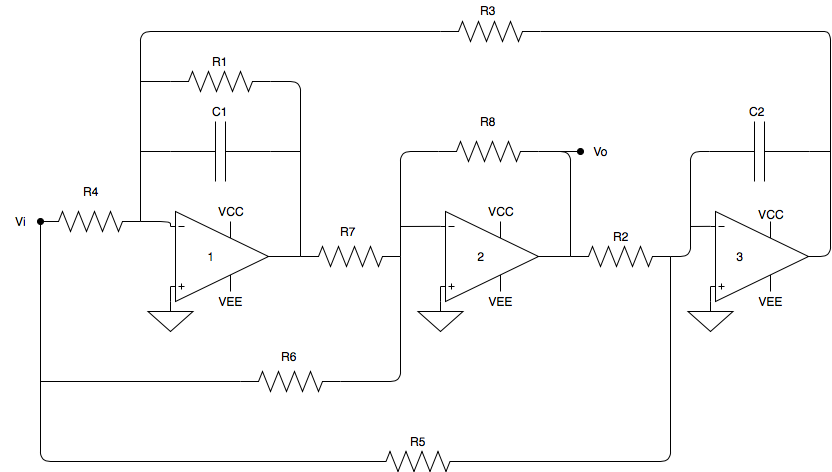
\includegraphics[width=12cm,height=12cm,keepaspectratio]{../EJ4/imagenes/FLEISCHER.png}
	\caption{Celda Fleischer-Tow}
	\label{fleischer2}
\end{figure}

\begin{table}[H] %estas son las del libro!
	\centering
	\begin{tabular}{c c c c c c c}
		Salida & Condiciones & $H(s)$ & $G$ & $\omega_p$ & $Q$ & $\omega_z$\\
		\hline \\
		BR (notch) &$R_1R_6=R_4R_7$ &\multirow{2}{*}{$- \frac{\frac{R_8}{R_6}s^2+\frac{R_8}{R_3R_5R_7C_1C_2}}{s^2+\frac{1}{R_1C_1}s+\frac{R_8}{R_2R_3R_7C_1C_2}}$}&\multirow{2}{*}{$-\frac{R_2}{R_5}$}& \multirow{2}{*}{$\sqrt{\frac{R_8}{R_2R_3R_7C_1C_2}}$}&
		\multirow{2}{*}{$R_1C_1\sqrt{\frac{R_8}{R_2R_3R_7C_1C_2}}$}
		&\multirow{2}{*}{$\sqrt{\frac{R_6}{R_3 R_5 R_7 C_1 C_2}}$}\\ \\ \\
		\hline
	\end{tabular}
	\caption{Caracter\'isticas de la celda Fleischer-Tow.}
	\label{f_cars}
\end{table}

Para los capacitores se comenz\'o por definir $C_1 = C_2 = 100nF$ ya que tendr\'ian el mismo valor que los capacitores de desacople. Sin embargo, de esta forma se obten\'ia un valor de $R_3$ muy chico, y dado que $C_1$ y $C_2$ forman parte del denominador de la expresi\'on de $R_3$, se termin\'o modificando sus valores a $1nF$. De esta forma $R_3$ tendr\'ia un valor del orden de los $k\Omega$ y los capacitores seguir\'ian con valores iguales.
En cuanto a las resistencias, se tuvo en cuenta la ganancia G, la frecuencia $\omega_0$ y el $Q$. Para ganancia unitaria, se eligi\'o: $R_2 = R_5 = 1k\Omega$.
\todo{SEGUIIIIIIR}

\subsubsection{Simulaci\'on y verificaci\'on}

\subsubsection{Dise\~o de PCB}

\subsubsection{Resultados obtenidos}

\subsection{Conclusiones} 
